\begin{figure}[h]
\hspace*{-8mm}
\begin{tikzpicture}
  \node (circ) {
    \begin{tikzpicture}
      \node[inner sep=0pt] (circuit) {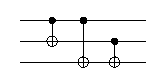
\includegraphics[scale=2]{Figures/circuits/bothEndsSimple}};  
      \node[above left=4.5mm and -7mm of circuit.west, opacity=0.9] {\footnotesize \(A\)};
      \node[left=-7mm of circuit.west, opacity=0.9] {\footnotesize \(B\)};
      \node[below left=4.5mm and -7mm of circuit.west, opacity=0.9] {\footnotesize \(C\)};
      \node[above right=0.8mm and 12.8mm of circuit.west, opacity=0.9] {\footnotesize \(\alpha\)};
      \node[below right=0.8mm and 23.6mm of circuit.west, opacity=0.9] {\footnotesize \(\beta\)};
      \node[below right=0.8mm and 34.4mm of circuit.west, opacity=0.9] {\footnotesize \(\gamma\)};
      \node[right=-3mm of circuit.north west, font=\itshape] (text) {a)};
    \end{tikzpicture}
  };
  \node[below right=-40mm and 20mm of circ] (hypergraph) {
    \begin{tikzpicture}
      \coordinate (O) at (0,0);
      \coordinate (auxA) at (90:9mm);
      \coordinate (auxC) at (330:9mm);
      \coordinate (A) at (90:18mm);
      \coordinate (B) at (210:18mm);
      \coordinate (C) at (330:18mm);
      \coordinate (a) at (270:9mm);
      \coordinate (b) at (30:9mm);
      \coordinate (c) at (150:9mm);
      \draw (auxA) -- (A);
      \draw (auxA) -- (b);
      \draw (auxA) -- (c);
      \draw[ultra thick] (auxC) -- (C);
      \draw[ultra thick] (auxC) -- (b);
      \draw[ultra thick] (auxC) -- (a);
      \draw (B) -- (a);
      \draw[ultra thick] (B) -- (c);
      \node[circle, right=-2.5mm of A, fill=white, inner sep=0pt, minimum size=5mm] {\(A\)};
      \node[circle, right=-2.5mm of B, fill=white, inner sep=0pt, minimum size=5mm] {\(B\)};
      \node[circle, right=-2.5mm of C, fill=white, inner sep=0pt, minimum size=5mm] {\(C\)};
      \node[circle, right=-2.5mm of a, fill=white, inner sep=0pt, minimum size=5mm] {\(\gamma\)};
      \node[circle, right=-2.5mm of b, fill=white, inner sep=0pt, minimum size=5mm] {\(\beta\)};
      \node[circle, right=-2.5mm of c, fill=white, inner sep=0pt, minimum size=5mm] {\(\alpha\)};
      \coordinate (joinPoint) at (30:15.5mm);
      \coordinate (leftPoint) at (300:16mm);
      \pic (cut) {cut=leftPoint/joinPoint};
      \coordinate (leftPoint2) at (120:16mm);
      \pic (cut2) {cut=leftPoint2/joinPoint};
      \coordinate (extraPoint) at (30:23.5mm);
      \pic (cut3) {cut=extraPoint/joinPoint};
      \node[above left=0mm and 13mm of A, font=\itshape] (text) {b)};
    \end{tikzpicture}
  };
  \node[below right=5mm and -70mm of circ] (distributed) {
    \begin{tikzpicture}
      \node[inner sep=0pt] (circuit) {
\includegraphics[scale=2]{Figures/circuits/farCNOTDistrib}};  
      \pic (e1) {ebit=e1/12.7mm/13mm};
      \pic (e2) {ebit=e2/33.84mm/13mm};
      \node[above left=18.58mm and -7mm of circuit.west, opacity=0.9] {\footnotesize \(A\)};
      \node[left=-7mm of circuit.west, opacity=0.9] {\footnotesize \(B\)};
      \node[below left=18.58mm and -7mm of circuit.west, opacity=0.9] {\footnotesize \(C\)};
      \node[above right=0.8mm and 65.8mm of circuit.west, opacity=0.9] {\footnotesize \(\alpha\)};
      \node[below right=0.8mm and 76.6mm of circuit.west, opacity=0.9] {\footnotesize \(\beta\)};
      \node[below right=0.8mm and 87.4mm of circuit.west, opacity=0.9] {\footnotesize \(\gamma\)};
      \coordinate[above left=10.5mm and -5mm of circuit.west] (leftPoint1);
      \coordinate[right=142mm of leftPoint1] (rightPoint1);
      \pic (cut1) {cut=leftPoint1/rightPoint1};
      \coordinate[below left=10.5mm and -5mm of circuit.west] (leftPoint2);
      \coordinate[right=142mm of leftPoint2] (rightPoint2);
      \pic (cut2) {cut=leftPoint2/rightPoint2};
      \node[right=-3mm of circuit.north west, font=\itshape] (text) {c)};
    \end{tikzpicture}
  };
\end{tikzpicture}
\caption{Distribution of circuit \textit{a)} when each wire is in a different QPU. Gate \(\beta\) is implemented as an `external' CNOT, i.e.\ both its control and target are in a remote QPU. The three non-local CNOTs only need two ebits in total, as \(\alpha\) and \(\gamma\) can use the ebits \(\beta\) requires.}
\label{fig:farCNOT}
\end{figure}